\documentclass{article}
\usepackage{tikz}

\begin{document}

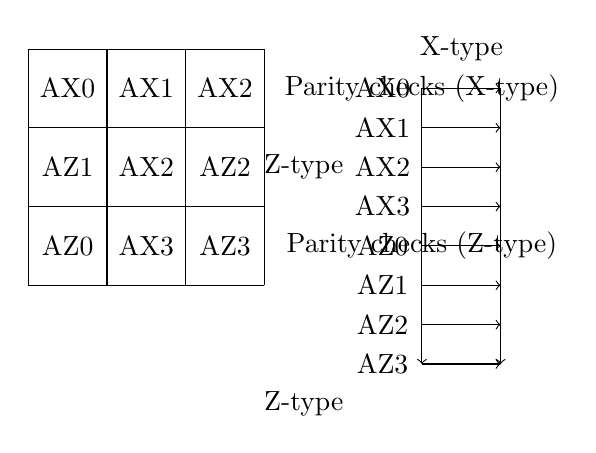
\begin{tikzpicture}

% Grid and labels
\draw (0,0) grid (3,3);
\node at (0.5,2.5) {AX0};
\node at (1.5,2.5) {AX1};
\node at (2.5,2.5) {AX2};
\node at (0.5,1.5) {AZ1};
\node at (1.5,1.5) {AX2};
\node at (2.5,1.5) {AZ2};
\node at (0.5,0.5) {AZ0};
\node at (1.5,0.5) {AX3};
\node at (2.5,0.5) {AZ3};

% Parity checks
\node[align=center] at (5,2.5) {Parity checks (X-type)};
\node[align=center] at (5,0.5) {Parity checks (Z-type)};

% Data
\begin{scope}[xshift=4cm]
\node at (0.5,2.5) {AX0};
\node at (0.5,2) {AX1};
\node at (0.5,1.5) {AX2};
\node at (0.5,1) {AX3};
\node at (0.5,0.5) {AZ0};
\node at (0.5,0) {AZ1};
\node at (0.5,-0.5) {AZ2};
\node at (0.5,-1) {AZ3};

\foreach \y in {2.5,2,1.5,1,0.5,0,-0.5,-1} {
  \draw[->] (1, \y) -- (2, \y);
}

\foreach \x in {1,2} {
  \draw[->] (\x, 2.5) -- (\x, -1);
}

\node at (1.5,3) {X-type};
\node at (-0.5,1.5) {Z-type};
\node at (-0.5,-1.5) {Z-type};

\end{scope}

\end{tikzpicture}
\end{document}